\section{R1: Idle Profiling for Scale-up Architectures}
\label{sec:idleprofile}

\begin{figure}[t]
\centering
\input{data/exim}
\caption{
  \exim throughput (i.e., delivering messages)
  with four file systems.
  To avoid I/O devices being scalability bottlenecks, we ran test
  clients on the same machine using \mem.
  We found that the manycore scalability of \exim
  depends a lot on the file systems
  (e.g., \ext is 54\x faster than \btrfs at 80-core).
  In particular, \btrfs spends 47\% of CPU time on synchronization;
  \ffs has been blocked (i.e., idle) for 95\% of its running time.
}
\label{f:exim}
\vspace{-5px}
\end{figure}

With the proliferation of fast IO devices as well as the increasing
core count in these systems, it is becoming difficult for developers
to identify scalability bottlenecks, as they are unexpected,
or worse yet, counter-intuitive in many cases.
%
For example, \autoref{f:exim} shows the scalability of the \exim mail
server with a varying number of cores on four widely deployed
file systems in our previous work~\cite{min:fxmark}.
%
Even though \exim is an embarrassingly parallel workload by design,
which does not have any bottleneck in delivering messages itself,
its scalability behavior is mainly dominated
by the characteristics of the underlying file systems.

One might consider using existing profiling tools~\cite{perflinux:web,
  lockstat:web, latencytop:web, bcc:web, vtune:web,
  hpctoolkit:ppopp10, hpctoolkit:web}
to understand the scalability problem in detail,
but unfortunately,
they cannot, by design,
produce an informative report
to explain the scalability bottlenecks in detail.
%
\autoref{t:prof-tools} summarizes the problem of existing profiling tools.
They are
limited in finding hotspots burning CPU cycles (\perf~\cite{perflinux:web}),
or provide insufficient information at both the kernel and userspace levels
(kernel lock-stat~\cite{lockstat:web}, LatencyTOP~\cite{latencytop:web},
off-CPU analysis in BCC toolkit~\cite{bcc:web},
Intel VTune~\cite{vtune:web},
HPCToolkit~\cite{hpctoolkit:ppopp10, hpctoolkit:web}).
%
For example, in \autoref{f:exim},
existing tools report either that CPUs are mostly idle during the benchmark
(e.g., sleeping routine in \ffs)
due to {\em blocking synchronization} such as mutex,
or that CPUs are utilized
(e.g., a spin loop in \btrfs)
due to {\em non-blocking synchronization} such as spinlock.
%
These two observed behaviors are barely useful for
developers to understand
why the profiled program does not scale well.
%
In addition, system-wide profiling, including user applications and
the OS kernel, is essential to discover such unexpected bottlenecks, but most
existing tools are designed to profile one or the other.


\begin{table}[tb]
\centering
\scriptsize
\begin{tabular}{lcccccc}
\toprule
\multirow{2}{*}{Profile tool} &
 \multicolumn{2}{c}{Profiling boundary} &
 \multicolumn{2}{c}{Profiling blocking sync.} &
 \multicolumn{2}{c}{Profiling non-blocking sync.} \\
 \cmidrule(l){2-3}
 \cmidrule(l){4-5}
 \cmidrule(l){6-7}
&
 User    & Kernel &
 Waiting task & Holding task &
 Waiting task & Holding task \\
\midrule
{Linux \perf} &
 \V & \V &
 -  & -  &
 -  & -  \\
{LatencyTOP}  &
 - & \V &
 \V & -  &
 -  & -  \\
{bcc off-CPU} &
 \V & \V &
 \V & -  &
 -  & -  \\
{Kernel Lock-stat} &
 - & \V &
 \V & -  &
 \V & -  \\
{Intel VTune Lock-Wait} &
 \V & - &
 \V & - &
 \V & -  \\
{HPCToolkit*}  &
 \V & - &
 \V & \V &
 \V & \V \\
\midrule
\textbf{Idle profiler}  &
 \V & \V &
 \V & \V &
 \V & \V \\
\bottomrule
\end{tabular}


  \vspace{0.5em}
  NOTE: HPCToolkit only supports profiling the \cc{pthread} library.
\caption{
  Comparison of existing profiling tools and our idle profiler.
  None of the existing tools provides sufficient information to correctly
  find scalability bottlenecks. Though HPCToolkit provides the richest
  information among the existing tools, its design is specific to
  \cc{pthread} libraries (i.e., spinlock and mutex) and incurs high
  runtime overhead due to its instrumentation. Unlike the existing
  profiling tools, our profiler is designed to provide
  system-wide information, which is sufficient for
  developers to easily understand scalability bottlenecks.
}
\label{t:prof-tools}
\vspace{-5px}
\end{table}

We will develop an {\em idle profiler} that will profile a system's idle
state to discover scalability bottlenecks in scale-up
architectures. Our goal is to perform system-wide profiling including kernel
and user applications with low performance overhead as well as no
source code modification.
This will allow us to find subtle performance bottlenecks. To this end,
as illustrated in~\autoref{f:idleprofiler-overview},
the idle profiler first finds spin loops by analyzing the binary
(\autoref{sub:spinfinder}) and then dynamically monitors various critical
sections that may contribute to the performance (\autoref{sub:dks}),
and finally suggests optimization candidates by analyzing the profiled results
offline (\autoref{sub:idlegraph}).
In this section, we describe our preliminary design decisions
along with the technical challenges.

\subsection{R1.1 Finding Non-blocking Synchronization Primitives}
\label{sub:spinfinder}

Identifying non-blocking synchronization primitives (e.g., spinlock,
spinning barrier) in a program is an essential step to profile wasted
CPU cycles for contending critical sections. At first glance, it looks
very simple---just find \cc{pthread_spin_lock()} and
\cc{pthread_barrier_wait()}.
%
But this is not the case in practice. Many performance-critical software
(e.g., MySQL~\cite{mysql:web}, RocksDB~\cite{rocksdb:web}, and the Linux kernel) 
and libraries (e.g., Intel TBB~\cite{tbb:web}, Boost C++
libraries~\cite{boost:web}, and Concurrency Kit~\cite{ck:web}) 
use their own non-blocking synchronization primitives
customized and optimized for their needs.
One common yet essential optimization
is inlining synchronization routines
either by declaring them as inline functions or macros. 
For example, MySQL uses three custom synchronization primitives (e.g.,
\cc{rw_lock_s_lock_spin()}), all of which
are inlined so they are distributed in more than a thousand places
in the compiled binary.
%
As a result, such an optimization as a result produces imprecise,
often complicated profiling results
(e.g., synchronization routines are mingled with their callers).
%
Potential solutions might be manual or dynamic instrumentation of
non-blocking synchronization primitives so that the profiler can monitor
each operation on the primitives. But such instrumentation-based
approaches impose high runtime overhead, which sometimes leads to
the dissappearance of the scalability bottlenecks (i.e., Heisenbug), or
seriously limits their applicability (e.g., dynamic instrumentation of
the operating system's kernel is challenging).

\boxbeg
\begin{Challenge}
  Non-blocking synchronization primitives are often inlined with their
  caller functions to avoid function call overhead. In that case,
  there is no function call of non-blocking synchronization
  primitives. What is the best way to discover non-blocking
  synchronization primitives in a program that is practical and
  provides reasonable performance without limiting the idle profiler's
  applicability?
\end{Challenge}
\boxend

We propose to find spinning loops in non-blocking synchronization
primitives by analyzing the program binary.
First, we assume that these binaries are running on shared memory
processor (SMP) architectures that are the most widely deployed ones.
Thus, for the non-blocking synchronization primitives, our approach
relies on the following property:

\vspace{1px}
\begin{itemize}
\item[]
\textbf{Spin Loop Property:}
{\em
  Non-blocking synchronization primitives have one or more spin loops,
  whose exit conditions (i.e., synchronization variables)
  are triggered by the external entity (i.e., other tasks) are outside of
  the loop.}
\end{itemize}
\vspace{1px}

Both the spinlock and spinning barrier follow the \textit{spin loop property}.
In the case of spinlock, lock waiters spin inside the loop until a lock holder
changes its {\em lock variable} to release the spinlock;
while in the spinning barrier, the last task hitting a barrier resets its {\em
barrier flag} to make previously arrived, waiting tasks proceed.

To be practical, the idle profiler should
perform system-wide profiling for both the kernel and the user
applications without modifying source code.
To meet this goal, we will analyze binary files to find such a spin loop and
its synchronization variable.
Specifically, we reconstruct a control
flow graph (CFG) from a disassembled binary file, and then find natural loops
in the CFG.
Among the identified loops, we select such loops that follow the spin loop
property, as spin loops, which are part of non-blocking
synchronization primitives. Also, for identified spin loops, we find
the definitions of synchronization variables for dynamic profiling
(\autoref{sub:dks}).
%
However, the binary analysis imposes research and engineering
challenges. For example, the analysis time should be reasonably small,
which is typically not the case with existing
approaches. Moreover, the obtained results should be precise so
the profiled results are correct. Even if that is not the case, the
dynamic profiling should be robust enough to filter out those cases.

\subsection{R1.2 Dynamic Profiling of Critical Sections}
\label{sub:dks}

\begin{figure}[t]
\centering
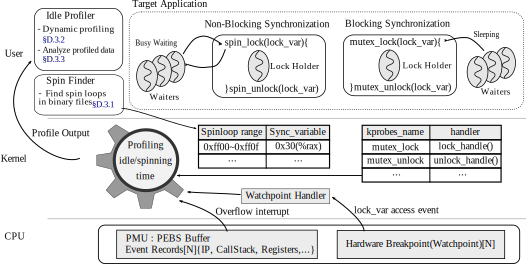
\includegraphics[width=0.90\textwidth]{fig/idleprofiler-dynsync}
\caption{
  The overall architecture of idle profiler, which profiles all kinds
  of synchronization primitives regardless of their running mode
  (kernel or user), types (blocking or non-blocking), and the role of
  tasks (waiter or holder). First, idle proiler analyzes the target
  binary files to find spinning loops that are part of the non-blocking
  synchronization primitives (\autoref{sub:spinfinder}). This is a one time
  job and the extracted spin loop information is cached for future uses.
  Its dynamic profiling mechanism uses the spin loop
  information to profile non-blocking synchronization primitives and
  monitors scheduling boundaries to profile blocking synchronization
  primitives (\autoref{sub:dks}). To reduce runtime overhead,
  it uses hardware performance monitoring features including precise
  event-based sampling (PEBS) and hardware watch-point. The profiled
  data will be used to get an idle graph that represents relations
  among critical sections (\autoref{sub:idlegraph}).
}
\label{f:idleprofiler-overview}
\vspace{-5px}
\end{figure}

\boxbeg
\begin{Challenge}
  In order to provide sufficient information to find scalability
  bottlenecks in a program, the idle profiler should achieve the
  following five goals:
  1) system-wide profiling across the whole software stack including
  user applications and OS kernel 2) for both blocking and non-blocking
  synchronization primitives, 3) that can not only find relations among
  waiting tasks and holding tasks, 4) but also have low profiling overhead
  to find subtle scalability bottlenecks, 5) with no source code modification
  to allow tapping into a real problematic / production environment.
  The challenge lies in achieving all of these goals together
  (for example, low profiling overhead vs. no source code modification).
\end{Challenge}
\boxend

To achieve all of the above goals, we plan to use the following
techniques in the dynamic monitoring of the idle profiler:
1) Instead of profiling each activity of every critical section, we
  will sample only contending ones to reduce profiling overhead;
2) Whenever possible, the profiling activities take place when a
  task is idling. This can effectively hide the profiling overhead;
3) Instead of directly modifying the source code or dynamically instrumenting
  binary files, we will extract necessary information in advance
  (\autoref{sub:spinfinder}) and use a probing mechanism, such as
  \kprobe~\cite{kprobes:doc}, to monitor activities without modifying
  source code.
In the rest of this section, we present in more detail our approach
and preliminary design for both non-blocking and blocking synchronization.

\PP{Non-blocking Synchronization.}
In the dynamic profiling of non-blocking synchronization primitives, we rely on the
spin loop property.
This property states that a non-blocking synchronization primitive has one or more
spin loops, whose exit condition is triggered by another task that is outside
those spin loops.
Thus, a task that spins on those identified spin loops is a waiting task,
whereas the one that triggers the exit condition (i.e., synchronization
variable) is a lock-holding task or a last-arriving task in a spinning
barrier.
\footnote{For brevity, we will simply say a lock holder or lock holding task.}

To detect such spinning tasks with low runtime overhead and without
modifying source code, we will use a hardware performance profiling
feature, Precise Event Based Sampling
(PEBS)~\cite{intel:sys-guide}. In particular, we will track the
exeuction of the conditional branch instructions that are essential in
any loop. We sample the execution of conditional branch using PEBS and
check whether or not its instruction pointer belongs to the pre-identified
spin loops. If so, that running task is a waiting task.

We can find a lock-holding task by finding a task that triggers the
exit condition of a spin loop. When a waiting task is found, we set a
hardware watchpoint~\cite{watchpoint:ols2009} to the
synchronization variable of the spin
loop, which is also pre-identified in~\autoref{sub:spinfinder}. After
setting the watchpoint, any task that writes to the memory address
will be trapped. If the trapped instruction pointer is not the spin
loops (i.e., a task triggers the exit condition of the spin loop), the
running task is a lock holder and is about to release the lock (or the
last task of a spinning barrier just arrived). Thus, we can associate
waiting tasks and holding tasks using the memory address of the
synchronization variable.
There are some design challenges here
since the number of hardware watchpoints is limited (e.g., four in
Intel x86 processors).

\PP{Blocking Synchronization.}
The waiting tasks of a blocking synchronization primitives go to the sleep
state by the task scheduler of the OS kernel. When a holding task releases
a lock, it wakes up one of the waiting tasks to pass over the lock. Thus,
monitoring scheduling boundaries in the kernel is one obvious way to
find critical sections by block synchronization primitives. However, simply
monitoring all scheduling activities will globally inhibit the
performance of the whole system.
For example, in our preliminary evaluation, the \cc{BCC's off-CPU}
analysis, which monitors all scheduling activities, decreased the
throughput of a multi-threaded key-value store, RocksDB, by
70\%. Thus, monitoring all task switch events is not viable to
meet the requirements of low-performance overhead on a production
system. One potential solution is monitoring task switch events only from known
callers using \kprobe. In fact, all user-level blocking
synchronization primitives either use \cc{pthread mutex} that relies on
\cc{futex} system call, or have their own implementation that has a spin
loop composed of a \cc{yield} system call.

%\if 0 Moreover, according to our preliminary experiments described in
%~\autoref{t:prof-overhead}, performance overhead of the existing toos are
%ranging from 25\% to 70\%.
%
%\begin{table}
%\centering
%\scriptsize
%\input{fig/tbl-profile-overhead}
%\caption{Benchmark results of the DB_BENCH(RocksDB)
%	by running 64 threads with various profiling tools.
%\label{t:prof-overhead}
%\end{table}
%\fi

\subsection{R1.3 Constructing an Idle Graph and Finding Optimization Candidates}
\label{sub:idlegraph}

\boxbeg
\begin{Challenge}
  In scale-up systems with many CPU cores, applications are becoming complex
  to fully utilize the parallelism using fine-grained locking.
  Thus, there are complex interactions among critical
  sections. In such cases, it is challenging to understand the
  overall scalability behavior of an application even after having the profiled
  results. Then, what is the best way to present the result of idle
  profiler that helps developers to easily understand the interactions among
  critical sections and provide better optimization candidates?
\end{Challenge}
\boxend

Existing profilers shown in~\autoref{t:prof-tools} merely show
profiled results ranked by accumulated waiting time. This might be
helpful to find simple bottlenecks.
When bottlenecks have complex dependencies among each other,
simple ranking-based analysis could be misleading.
Thus, it is necessary to analyze comprehensive relationship among bottlenecks
to help developers deeply understand the scalability behavior of an
application.

For developers to easily understand relations among critical sections
and their impact on scalability, we will further analyze profiled data
and present a graph of critical sections and their waiting and holding
tasks, named an {\em idle graph}, by analyzing holder-waiter relation
in the profiled data. The idle profiler's profile data will contain
task information (e.g., process/thread id), waiting/holding time, and
the call stack of lock acquire/release point. It also has a waiter
list of a lock holder to draw the idle graph.
%
We will perform offline analysis on profiled data to get an idle
graph. As \autoref{f:idleprofiler-idlegraph} shows, the idle graph
will be a directed acyclic graph (DAG), that consists of a call stack
as a vertex, and connections between a lock holder and a waiter as
edges. Each vertex has an weight that shows accumulated time for
waiting or holding.
%
In addition, we will plan to explore to estimate the optimization
impact of a critical section that can suggest the optimization
candidates to developers.

\begin{figure}[!t]
\centering
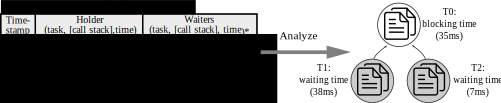
\includegraphics[width=0.80\textwidth]{fig/idleprofiler-idlegraph}
\caption{Example of an idle graph. We create an idle graph by
  analyzing the profiled data. An idle graph represents the relationships
  among critical sections and their waiting and holding tasks.
  The vertex \cc{T0}, \cc{T1}, and \cc{T2} represent call stacks of
  holding and waiting tasks, respectively. The edges show
  holder-waiter relation between the blocker's stack \cc{T0} and the
  waiter's stack \cc{T1} and \cc{T2}.}
\label{f:idleprofiler-idlegraph}
\vspace{-5px}
\end{figure}


